\def\makeitoi{
    \section{Mô hình Multimodal Unsupervised Image-to-Image Translation}
    
    \subsection{Bài toán Image-to-Image Translation}
    Image-to-Image Translation\index{Image-to-Image Translation} (viết tắt là I2I\index{I2I}) là một bài toán trong lĩnh vực computer vision nhắm đến việc biến đổi các thuộc tính của ảnh ban đầu để thu được một ảnh khác theo từng nhu cầu hay nói cách khác là ta cần huấn luyện mô hình sao cho có thể ánh xạ một ảnh đầu vào tương ứng với một ảnh đầu ra. Các mô hình giải bài toán I2I nhận đầu vào là một ảnh, và đưa đầu ra là một cách theo từng yêu cầu cụ thể của bài toán. Thông thường thì ảnh đầu vào và ảnh đầu ra của các mô hình I2I là các ảnh cùng kích thước nhưng khác nhau về  các thuộc tính trong ảnh. Ví dụ: ảnh không màu và ảnh có màu, ảnh người chụp và ảnh hoạt hình, ảnh mờ và ảnh nét, ảnh màu được chuyển sang cách tô màu theo cách phong cách khác như của Monet hay Van Gogh. 
    \begin{figure}[H]
    \centering
    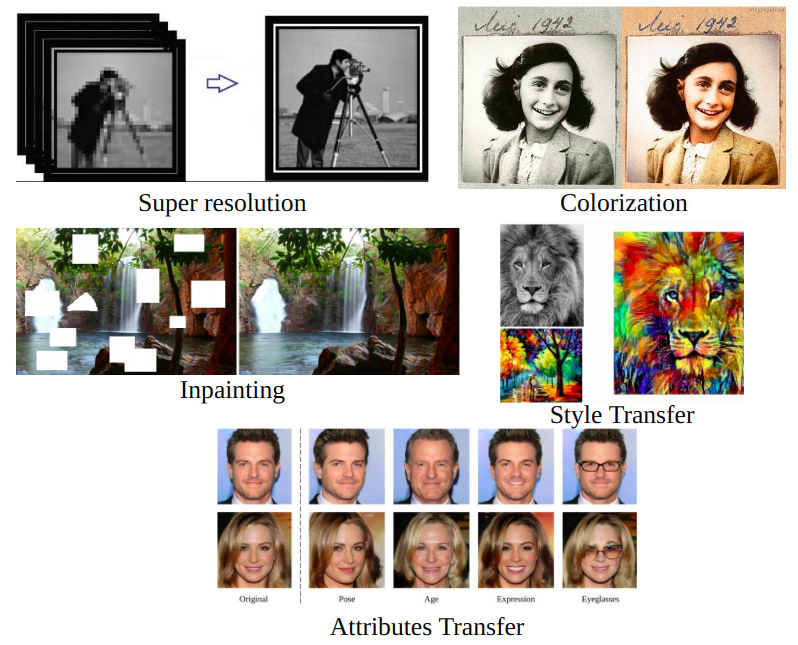
\includegraphics[width=10cm]{images/i2i_problems.png}
    \caption{Các bài toán nhỏ nằm trong bài toán Image-to-Image Translation (Nguồn: Internet)}
    \label{fig:img_problems}
    \end{figure}
    \noindent Từ đó, một số bài toán nhỏ của I2I có thể nhắc đến là:
    \begin{itemize}[leftmargin=0cm,itemindent=.5cm,labelwidth=\itemindent,labelsep=0cm,align=left]
        \item Super resolution\index{super resolution}: Biến đổi một ảnh có kích thước nhỏ thành một ảnh có kích thước lớn hơn
        \item Colorization\index{colorization}: Tô màu ảnh
        \item Inpainting\index{inpainting}: Điền vào chỗ trống trong ảnh
        \item Style transfer\index{style transfer}: Biến đổi ảnh ban đầu theo style của ảnh khác
        \item Attribute transfer\index{attribute transfer}: Chuyển thuộc tính của ảnh này sang ảnh khác
    \end{itemize}
    \noindent Nếu bộ dữ liệu bao gồm các cặp ảnh (hai ảnh có cùng nội dung nhưng thuộc hai domain khác nhau), bài toán I2I có thể được giải quyết bằng một số mô hình supervised learning như ConditionalGan\index{ConditionalGan} \cite{conditional-gan}, Pix2Pix\index{Pix2Pix} \cite{high-resolution-conditional-gan}, BicycleGAN\index{BicycleGAN} \cite{bicyle-gan}. Tuy nhiên, trong một số trường hợp đặc biệt, ta không thể xây dựng được bộ dữ liệu theo cặp như trên (có thể kể đến bài toán chuyển đổi giữa ảnh nam và ảnh nữ, chuyển đổi giữa ảnh trẻ và ảnh già), ta cần những mô hình unsupervised learning\index{unsupervised learning}.\\
    Vì các mô hình supervised learning\index{supervised learning} yêu cầu bộ dữ liệu có từng cặp ảnh đầu vào và ảnh đầu ra tương ứng nên các mô hình đó sẽ được huấn luyện dễ hơn. Tuy nhiên, việc làm ra những bộ dữ liệu đó có thể tốn rất nhiều thời gian và công sức. Bên cạnh đó, những mô hình unsupervised learning không yêu cầu những bộ dữ liệu bao gồm các cặp dữ liệu mà ta chỉ cần hai nhóm dữ liệu riêng biệt nên việc chuẩn bị các bộ dữ liệu đó đơn giản hơn rất nhiều.

    \begin{figure}[H]
    \centering
    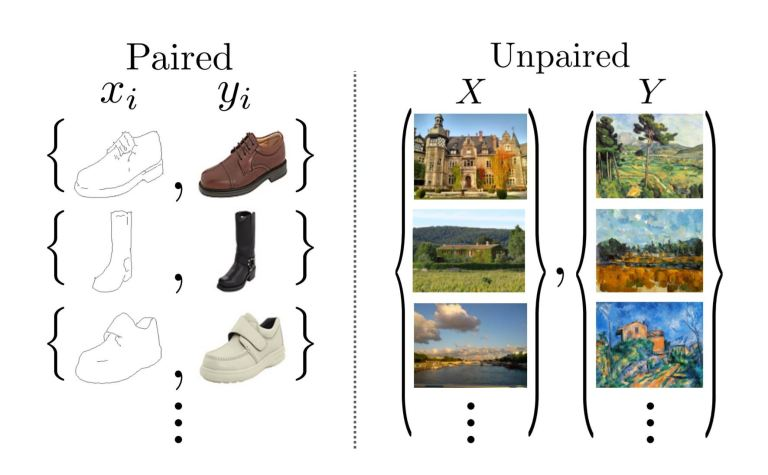
\includegraphics[width=10cm]{images/img_translation.jpg}
    \caption{Bộ dữ liệu theo cặp (trái), Bộ dữ liệu không theo cặp (phải) (Nguồn: \cite{cycle-gan})}
    \label{fig:img_translation}
    \end{figure}
    
    \noindent Bên cạnh vấn đề về dữ liệu, trong một số trường hợp cụ thể, từ một ảnh thuộc domain gốc, ta không chỉ muốn sinh ra một ảnh mà còn muốn sinh ra nhiều ảnh khác nhau thuộc domain mục tiêu. Ví dụ, trong việc chuyển đổi giữa ảnh mùa đông và ảnh mùa hè, một khung cảnh mùa đông có thể có nhiều khung cảnh tương ứng trong mùa hè dựa vào thời gian, ánh sáng ...  Từ đó, ta phân loại các mô hình thành hai nhóm mô hình unimodal và mô hình multimodal. Mô hình dạng unimodal là mô hình chỉ cho ra một ảnh đầu ra tương ứng với mỗi một ảnh đầu vào. Một số mô hình đã được đề xuất như CycleGAN \cite{cycle-gan}, DiscoGAN \cite{disco-gan}, UNIT \cite{unit} ... Mô hình dạng multimodal là mô hình cho ra được nhiều ảnh đầu ra với mỗi một ảnh đầu vào. Một số mô hình đã được đề xuất như BicycleGAN \cite{bicyle-gan}, DRIT++ \cite{drit-plus}, StarGAN \cite{star-gan} ... Rõ ràng, nếu có thể, sử dùng các mô hình multimodal sẽ cho ra được đa dạng ảnh thu được cho mỗi ảnh đầu vào.\\
    Để giải quyết cả hai vấn đề trên, năm 2018, Xun Huang và các cộng sự đã đề xuất mô hình Multimodal Unsupervised Image-to-Image Translation \cite{munit} (gọi tắt là MUNIT), vừa giải quyết vấn đề về các bộ dữ liệu không theo cặp (yêu cầu mô hình unsupervised learning), vừa giải quyết vấn đề về sinh ra nhiều ảnh đầu ra từ một ảnh đầu vào duy nhất (yêu cầu mô hình multimodal).

    \subsection{Ý tưởng chính}
    MUNIT hoạt động dựa trên một số giả thuyết:
    \begin{itemize}[leftmargin=0cm,itemindent=.5cm,labelwidth=\itemindent,labelsep=0cm,align=left]
        \item Đầu tiên, MUNIT giả sử rằng một ảnh có thể được encode vào hai không gian riêng biệt chứa những thông tin khác nhau của ảnh đó là content space\index{content space} và style space\index{style space}. Content space lưu giữ những thông tin về nội dung của bức ảnh (đường nét, khuôn hình của sự vật trong ảnh). Style space lưu giữ những thông tin về phong cách, đặc điểm của bức ảnh (màu sắc, hình dáng cụ thể của sự vật trong ảnh)
        \item Ngoài ra, MUNIT\index{MUNIT} giả sử rằng hai ảnh thuộc hai domain khác nhau dùng chung content space nhưng sử dụng hai style space khác nhau.
    \end{itemize}
    \noindent MUNIT biến đổi một ảnh từ domain này sang domain khác bằng cách sử dụng content code của ảnh đó kết hợp với style code được sinh ngẫu nhiên thuộc style space của domain đích. Content code chứa những thông tin của ảnh mà sẽ được giữ lại trong quá trình biến đổi và style code đại diện cho biến thể của ảnh trong domain đích. Bằng việc sinh ngẫu nhiên style code từ style space của domain đích, MUNIT đảm bảo đầu ra là multimodal\index{multimodal}.
    \begin{figure}[H]
    \centering
    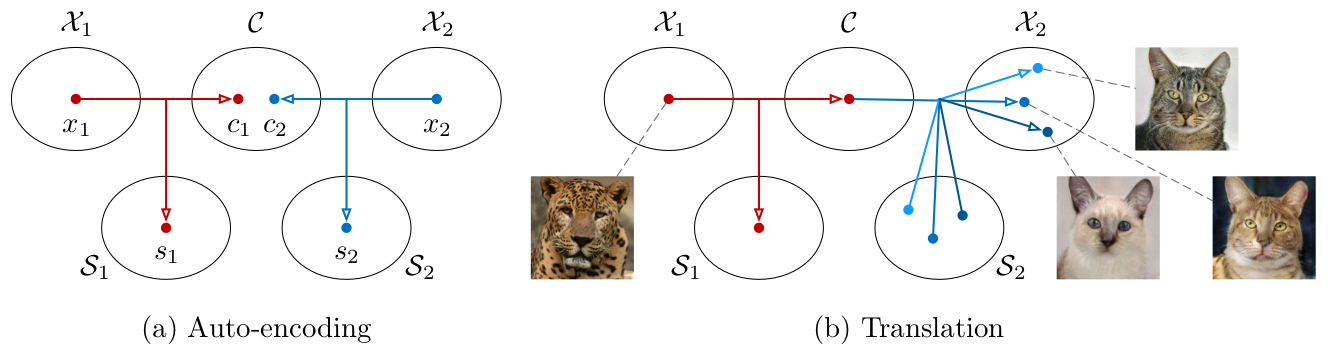
\includegraphics[width=12cm] {images/idea_munit.png}
    \caption{Ý tưởng của mô hình MUNIT (Nguồn: \cite{munit})}
    \label{fig:idea_munit}
    \end{figure}

    \subsection{Hệ thống các hàm loss}
    \noindent Mô hình MUNIT bao gồm hai loại hàm loss chính là Bidirectional reconstruction loss\index{Bidirectional reconstruction loss} và Adversarial loss\index{Adversarial loss} (hay còn gọi là GAN loss). Ngoài ra, MUNIT còn có Domain-invariant perceptual loss\index{Domain-invariant perceptual loss} có thể được tuỳ chọn sử dụng trong một số trường hợp nhất định.

    \begin{figure}[H]
    \centering
    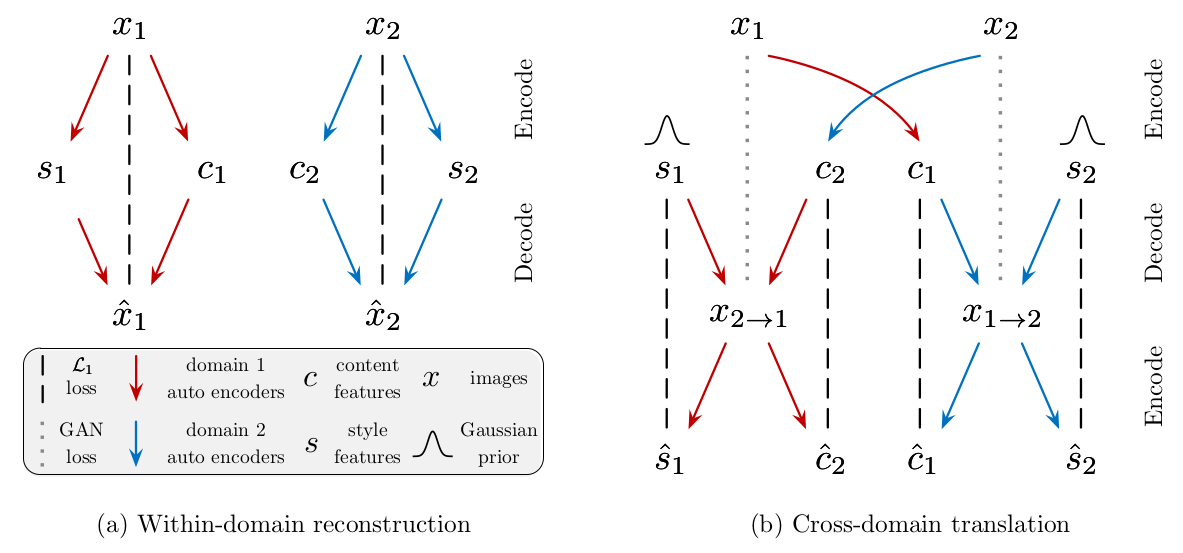
\includegraphics[width=12cm] {images/loss_munit.png}
    \caption{Hệ thống hàm loss của mô hình MUNIT (Nguồn: \cite{munit})}
    \label{fig:loss_munit}
    \end{figure}

    \noindent Trong phần này, các hàm loss sẽ được sử dụng một số ký hiệu như sau:
    \begin{itemize}[leftmargin=0cm,itemindent=.5cm,labelwidth=\itemindent,labelsep=0cm,align=left]
        \item $\mathcal{L}$: Hàm loss
        \item $\mathbb{E}$: Giá trị kỳ vọng
        \item E: Hàm đại diện cho Encoder
        \item G: Hàm đại diện cho Generator
        \item D: Hàm đại diện cho Discriminator
        \item ${x}_{i}$: Ảnh thuộc domain i
        \item $c$: Content của ảnh
        \item ${s}_{i}$: Style của ảnh thuộc domain i
    \end{itemize}

    \subsubsection{Hàm bidirectional reconstruction loss}
    Để xây dựng một mô hình auto-encoder\index{auto-encoder} trong đó quá trình encoder ngược với decoder và tương tự decoder là ngược với encoder, MUNIT xây dựng bidirectional reconstruction loss nhằm đảm bảo các quá trình: ảnh $\rightarrow$ latent $\rightarrow$ ảnh and latent $\rightarrow$ ảnh $\rightarrow$ latent. MUNIT sử dụng reconstruction loss là $\mathcal{L}_{1}$ loss. Bidirectional reconstruction loss bao gồm Image reconstruction loss\index{Image reconstruction loss} và Latent reconstruction loss\index{Latent reconstruction loss}.\\
    \textbf{- Hàm image reconstruction loss:} Hàm loss này có tác dụng trong việc xây dựng lại ảnh sau khi encode. Ảnh ban đầu và ảnh được sinh ra sau quá trình encode và decode trong cùng một domain phải giống nhau.
    \begin{align}
    \mathcal{L}^{x_{i}}_{1} = \mathbb{E}_{x_{i} \sim p(x_{i})}[||G_{i}(E_{i}^{c}(x_{i}), E_{i}^{s}(x_{i}))-x_{i}||_{1}]
    \end{align}
    \textbf{- Hàm latent reconstruction loss:} Hàm loss này có tác dụng trong việc xây dựng lại các latent code sau khi biến đổi ảnh từ domain gốc sang domain đích. Có hai loại Latent reconstruction loss là Content reconstruction loss $\mathcal{L}^{c_{i}}_{1}$ và Style reconstruction loss $\mathcal{L}^{s_{i}}_{1}$. Content reconstruction loss yêu cầu mô hình phải giữ được nội dung của ảnh sau khi biến đổi từ domain gốc sang domain đích. Style reconstruction loss yêu cầu mô hình sinh ra ảnh mới có style code đúng thuộc style space của domain đích.
    \begin{align}
    \mathcal{L}^{c_{i}}_{1} = \mathbb{E}_{c_{i}\sim p(c_{i}), s_{j}\sim q(s_{j})}[||E^{c}_{j}(G_{j}(c_{i},s_{j}))-c_{i}||_{1}]
    \end{align}
    \begin{align}
    \mathcal{L}^{s_{i}}_{1} = \mathbb{E}_{c_{j}\sim p(c_{j}), s_{i}\sim q(s_{i})}[||E^{s}_{i}(G_{i}(c_{j},s_{i}))-s_{i}||_{1}]
    \end{align}
    
    \subsubsection{Hàm adversarial loss}
    Hàm adversarial loss (hàm GAN loss) là hàm loss của Discriminator và có tác dụng trong việc giúp cho ảnh được sinh ra sau quá trình biến đổi dần dần giống với ảnh thật từ bộ dữ liệu. Tuy nhiên, khác với mô hình GANs gốc, MUNIT sử dụng LSGAN \cite{lsgan} trong vai trò adversarial loss nhằm cải thiện khả năng luyện của mô hình, tránh các vấn đề liên quan tới vanishing gradient. Chi tiết về LSGAN s
   ẽ được trình bày tại phần \ref{sec_lsgan}
    \begin{align}
    \mathcal{L}^{x_{j}}_{\text{GAN}} = \mathbb{E}_{c_{i} \sim p(c_{i}), s_{j} \sim q(s_{j})} [\log(1 - D_{j}(G_{j}(c_{i}, s_{j})))] + \mathbb{E}_{x_{j} \sim p(x_{j})} [\log D_{j}(x_{j})]
    \end{align}
    
    \subsubsection{Hàm Least Squares Generative Adversarial Networks\index{Least Squares Generative Adversarial Networks}}
    \label{sec_lsgan}
    Hàm loss \ref{func:gan_loss} được giới thiệu trong bài báo của Ian Goodfellow và các cộng sự dựa trên hàm binary cross entropy dành cho bài toán phân lớp nhị phân, do đó, tồn tại những điểm yếu.\\
    Trong quá trình huấn luyện mô hình GANs\index{GANs}, ở giai đoạn đầu, Generator\index{generator} gần như sinh ra những bức ảnh rất xấu và điều này khiến cho Discriminator\index{discriminator} dễ dàng phân biệt. Khi đó, giá trị đầu ra của Discriminator\index{discriminator} đối với ảnh sinh bởi Generator\index{generator} $D(G(z))$ tiến gần tới 0. Với tính chất của hàm kích hoạt sigmoid, điều này khiến cho đạo hàm lúc này gần như bằng 0, tương đương với việc gần như không có thông tin có ích nào được cập nhật vào cả hai thành phần. Quá trình này khiến cho mô hình GANs rơi vào trạng thái mất mát đạo hàm (vanishing gradient).\\
    Hàm Least Squares Generative Adversarial Networks (được gọi tắt là LSGAN\index{LSGAN}) được thiết kế để giảm thiểu tình trạng trên, giúp việc luyện mô hình GANs trở nên dễ dàng hơn.
    \begin{align}
    \min_D V_{\text{\tiny LSGAN}}(D) = &\frac{1}{2}\mathbb{E}_{\bm{x} \sim p_{\text{data}}(\bm{x})}\bigl[(D(\bm{x})-b)^2\bigr]+ \frac{1}{2}\mathbb{E}_{\bm{z} \sim p_{\bm{z}}(\bm{z})}\bigl[(D(G(\bm{z}))-a)^2\bigr]
    \end{align}
    \begin{align}
    \min_G V_{\text{\tiny LSGAN}}(G) = &\frac{1}{2}\mathbb{E}_{\bm{z} \sim p_{\bm{z}}(\bm{z})}\bigl[(D(G(\bm{z}))-c)^2\bigr]
    \end{align}
    trong đó:
    \begin{itemize}[leftmargin=0cm,itemindent=.5cm,labelwidth=\itemindent,labelsep=0cm,align=left]
        \item $x$ là điểm dữ liệu thật
        \item $D(x)$ là xác suất mà Discriminator\index{discriminator} dự đoán $x$ là dữ liệu thật
        \item $E_x$ là kỳ vọng đối với các giá trị của dữ liệu thật $x$
        \item $z$ là đầu vào ngẫu nhiên của Generator\index{generator}
        \item $G(z)$ là điểm dữ liệu được sinh ra bởi Generator\index{generator}
        \item $D(G(z))$ là xác suất mà Discriminator\index{discriminator} dự đoán $G(z)$ là dữ liệu thật
        \item $E_z$ là kỳ vọng đối với các giá trị ngẫu nhiên $z$
        \item $a$ và $b$ lần lượt là nhãn của ảnh sinh ra từ Generator và ảnh từ bộ dữ liệu trong quá trình luyện Discriminator
        \item $c$ là nhãn của ảnh sinh ra từ Generator trong quá trình luyện Generator
    \end{itemize}
    \begin{figure}[H]
    \centering
    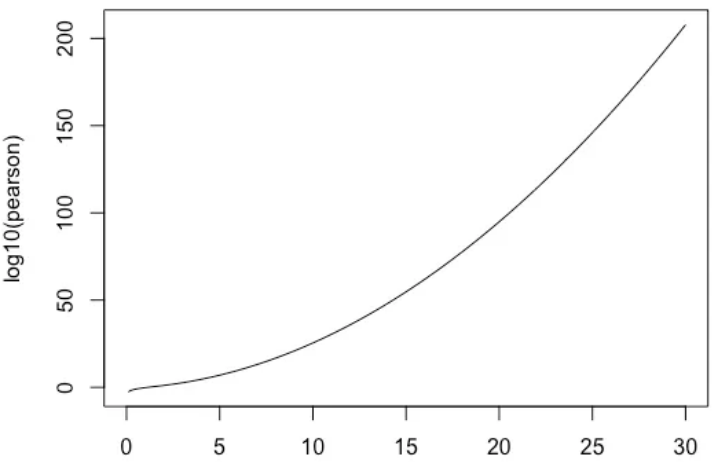
\includegraphics[width=5.5cm] {images/pearson.png}
    \caption{Đồ thị hàm Pearson $\chi^2$ divergence (Nguồn: nttuan8.com)}
    \label{fig:pearson}
    \end{figure}
    Một điều kiện đối với ba tham số a, b, c là b − c = 1 và b − a = 2 nhằm đưa 
    \begin{equation}
    \min_G V_{\text{\tiny LSGAN}}(G) = \chi^2_\text{Pearson}(p_\text{d}+p_g\|2p_g)
    \end{equation}
    trong đó $\chi^2_\text{Pearson}$  là Pearson $\chi^2$ divergence. Điều này đồng nghĩa với việc tối thiểu hoá hàm loss của Generator trong LSGAN là tối thiểu hoá Pearson $\chi^2$ divergence. Hàm Pearson $\chi^2$ divergence có đồ thị như Hình \ref{fig:pearson}, đảm bảo việc duy trì giá đạo hàm trên mọi giá trị.

    \noindent Để thoả mãn điều kiện trên, ta có thể chọn bộ ba số a = −1, b = 1, và c = 0, ta có hàm loss như sau:
    \begin{align}
    \min_D V_{\text{\tiny LSGAN}}(D) = &\frac{1}{2}\mathbb{E}_{\bm{x} \sim p_{\text{data}}(\bm{x})}\bigl[(D(\bm{x})-1)^2\bigr]+ \frac{1}{2}\mathbb{E}_{\bm{z} \sim p_{\bm{z}}(\bm{z})}\bigl[(D(G(\bm{z}))+1)^2\bigr]
    \end{align}
    \begin{align}
    \min_G V_{\text{\tiny LSGAN}}(G) = &\frac{1}{2}\mathbb{E}_{\bm{z} \sim p_{\bm{z}}(\bm{z})}\bigl[(D(G(\bm{z})))^2\bigr]
    \end{align}
    Vậy là LSGAN đã giải quyết vấn đề vaninshing gradient khi huấn luyện Generator\index{generator}. Ngoài ra, thực nghiệm cho thấy LSGAN có thể sinh ra ảnh chất lượng tốt hơn hàm loss mặc định của mô hình GANs cũng như ổn định hơn trong quá trình huấn luyện.
    
    \subsubsection{Tổng các hàm loss của mô hình}
    MUNIT tính tổng loss của mô hình bằng việc tính tổng có trọng số của các bidirectional reconstruction loss và adversarial loss.
    \begin{multline}
    \underset{E_{i}, E_{j}, G_{i}, G_{j}} \min \underset {D_{i}, D_{j}} \max \mathcal{L}(E_{i}, E_{j}, G_{i}, G_{j}, D_{i}, D_{j}) = \mathcal{L}^{x_{i}}_{\text{GAN}} + \mathcal{L}^{x_{j}}_{\text{GAN}} \\+ \lambda_{x}(\mathcal{L}^{x_{i}}_{\text{recon}} +  \mathcal{L}^{x_{j}}_{\text{recon}})
    + \lambda_{c}(\mathcal{L}^{c_{i}}_{\text{recon}} +  \mathcal{L}^{c_{j}}_{\text{recon}}) +  \lambda_{s}(\mathcal{L}^{s_{i}}_{\text{recon}} +  \mathcal{L}^{s_{j}}_{\text{recon}})
    \end{multline}
    trong đó $\lambda_{x}$, $\lambda_{c}$, $\lambda_{s}$ lần lượt là trọng số của mỗi giá trị hàm loss. Cụ thể, giá trị mặc định của $\lambda_{x}$ bằng 10, $\lambda_{c}$, $\lambda_{s}$ đều có giá trị bằng 1. Tác giả ưu tiên việc luyện cho mô hình có khả năng khôi phục lại ảnh trước khi có thể tạo ra ảnh mới.
    
    \subsubsection{Hàm domain-invariant perceptual loss}
    Một hàm loss phụ (có thể tùy chọn sử dụng hoặc không) trong MUNIT là Perceptual loss. Perceptual loss thường được tính bằng khoảng cách giữa các đặc trưng của ảnh sau khi đưa qua mô hình VGG. Đối với mô hình unsupervised learning, ta sẽ tính khoảng cách giữa các đặc trưng về content của ảnh đầu vào và ảnh đầu ra (ảnh đầu vào và ảnh đầu ra sau khi biến đổi phải có cùng content với nhau). Cụ thể, trước khi tính toán khoảng cách, tác giả sử dụng Instance Normalization đối với các đặc trưng đầu ra từ mô hình VGG nhằm xoá bỏ các đặc trưng về mean và standard deviation (chứa những đặc trưng về style). Tác giả cho rằng đối với ảnh chất lượng cao (kích thước từ 512x512 pixel trở lên) thì quá trình training được cải thiện đáng kể.
    
    
    \subsection{Chi tiết kiến trúc}
    Mô hình của MUNIT được chia thành các phần chính gồm hai bộ Generator\index{generator} và Discriminator\index{discriminator} tương ứng với mỗi domain. Generator của MUNIT\index{MUNIT} có kiến trúc theo dạng auto-encoder\index{auto-encoder} với Content Encoder\index{Content Encoder}, Style Encoder\index{Style Encoder} và Decoder\index{Decoder}.
    
    \begin{figure}[H]
    \centering
    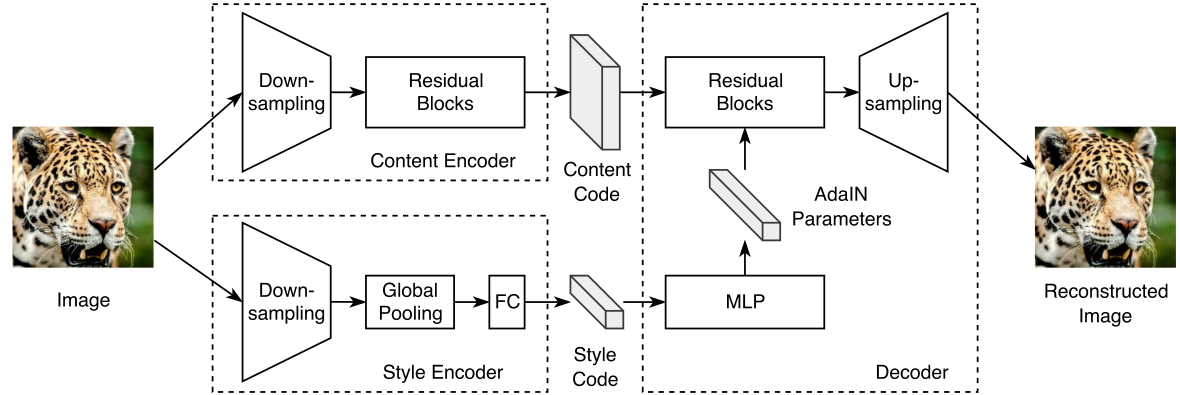
\includegraphics[width=13cm] {images/detail_munit.png}
    \caption{Chi tiết kiến trúc của Generator trong mô hình MUNIT (Nguồn: \cite{munit})}
    \label{fig:detail_munit}
    \end{figure}
    
    \subsubsection{Kiến trúc của Content Encoder}
    Content Encoder của MUNIT nhận đầu vào là ảnh và đưa đầu ra là content code chứa nội dung của ảnh (nội dung được bảo toàn qua quá trình biến đổi).\\
    Content Encoder bao gồm downsampling block và các residual block. Downsampling block có nhiệm vụ giảm kích thước về chiều dài và chiều rộng của ảnh đầu vào thông qua các layer convolution với stride bằng 2. Sau đó là các residual block (cụ thể trong cấu hình mặc định của MUNIT là 4 residual block) giúp giữ lại các đặc trưng liên quan đến nội dung của ảnh. Các layer convolution ở đây có stride bằng 1 và được padding nên kích thước chiều dài và chiều rộng của features map không đổi.\\
    Kiểu padding trong các layer convolution đều là reflection padding và activation function là ReLU. Trong Content Encoder, tác giả sử dụng Instance Normalization \cite{in} trong tất cả các layer convolution nhằm xoá bỏ các đặc trưng thống kê của ảnh (những đặc trưng liên quan đến style của ảnh). Điều này khiến cho content của các ảnh thuộc các domain khác nhau có thể được encode vào cùng một không gian theo đúng giả thuyết của mô hình.
    
    \subsubsection{Kiến trúc của Style Encoder}
    Style Encoder của MUNIT nhận đầu vào là ảnh và đưa đầu ra là style code đại diện cho style của domain của ảnh.\\
    Tương tự như Content Encoder, Style Encoder cũng bao gồm downsampling block giúp giảm kích thước của ảnh đầu vào thông qua một số layer convolution với stride. Sau đó là layer global pooling (cụ thể là global average pooling) giúp đưa features map về dạng vector trước khi đưa qua fully connected layer để thu được style code của ảnh. Kích thước style code của MUNIT có thể tuỳ biến, tuy nhiên, trong cấu hình mặc định của MUNIT, style code có kích thước là vector 8 chiều.\\
    Khác với Content Encoder, Style Encoder không dùng bất kỳ loại normalization nào sau các layer convolution. Mục tiêu của việc này là giúp cho Style Encoder giữ nguyên chính xác các đặc trưng thống kê của ảnh vào style code từ đó khiến cho style code mang đúng nhất các đặc trưng về style của ảnh.
    
    \subsubsection{Kiến trúc của Decoder}
    Decoder của MUNIT nhận hai đầu vào là content code từ Content Encoder và style code từ Style Encoder và đưa đẩu ra là ảnh theo domain từ style code đầu vào.\\
    Style code sẽ được đưa qua multilayer perceptron với mục tiêu là thu được hai giá trị mean và standard deviation của style đó và lấy đó làm tham số đầu vào của AdaIN layer. Content code được Decoder đưa qua một vài residual block. Trong đó, các layer convolution có stride bằng 1, padding kiểu reflection, normalization layer là AdaIN với các tham số đã được tính ở trên, activation function là ReLU.\\
    Features map thu được sau residual block được đưa qua upsampling block nhằm đưa các kích thước chiều dài và chiều rộng về đúng kích thước ảnh, số channel về 3 ứng với ảnh RGB. Mỗi upsampling block chứa 1 layer upsample theo phương pháp nearest neighbor và 1 layer convolution. Convolution layer có stride bằng 1, sử dụng padding theo kiểu reflection, activation là ReLU. Đáng chú ý là tác giả sử dụng Layer Normalization \cite{layer_norm} sau mỗi convolution layer trong upsampling block. Mục tiêu của việc này là nhằm giữ lại chính xác các đặc trưng về mặt thống kê của các features map, từ đó, giúp ảnh đầu ra thuộc chính xác domain tương ứng với style code đầu vào.

    \subsubsection{Kiến trúc của Discriminator}
    \noindent Discriminator trong MUNIT có kiến trúc multiscale giúp cho những thông tin discriminator cập nhật lại generator có khả năng định hướng generator tạo ra ảnh đúng về cấu trúc tổng quát (giữ nguyên được content của ảnh ban đầu) và tạo ra những chi tiết ảnh giống thật (biển đổi ảnh theo style mục tiêu).
    \begin{figure}[H]
    \centering
    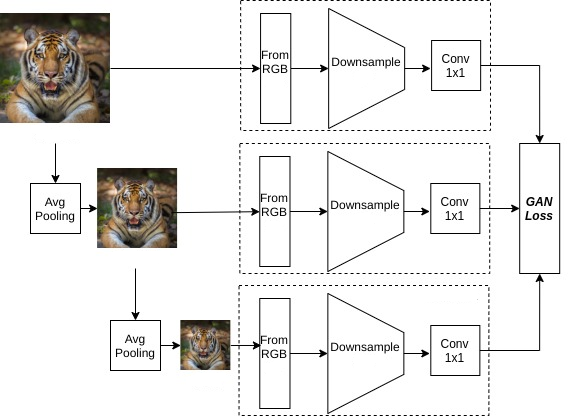
\includegraphics[width=10cm] {images/detail_dis.png}
    \caption{Chi tiết kiến trúc của Discriminator trong mô hình MUNIT}
    \label{fig:detail_dis}
    \end{figure}
    \noindent Trong cấu hình mặc định, discriminator gồm 3 block có kiến trúc giống nhau tuy nhiên chúng được luyện với các trọng số độc lập và nhận đầu vào có kích thước khác nhau. Đầu ra của 3 block trong discriminator được tính loss bằng hàm LSGAN và giá trị loss cuối cùng được tính trung bình trước khi dùng để cập nhật các trọng số của MUNIT.\\
    Mỗi block có 1 layer FromRGB là 1 layer convolution đưa số channel của ảnh đầu vào từ 3 (ảnh RGB) thành số channel như mong muốn. Sau FromRGB là downsampling block giúp giảm kích thước chiều dài và chiều rộng của ảnh. Các layer convolution đều sử dụng padding kiểu reflection, activation function là Leaky ReLU và không có normalization nhằm giữ nguyên các giá trị thống kê (đại diện cho style) của ảnh ban đầu.\\
    Mỗi ảnh đầu vào được giảm kích thước bằng average pooling layer trước khi được đưa vào một block khác của discriminator. Mỗi lần đi qua average pooling layer, chiều dài và chiều rộng của ảnh được giảm đi một nửa.\\
    Ngoài ra, một số bài báo \cite{lipschitz1}, \cite{lipschitz2} đã chứng minh rằng, nếu Discriminator trong mô hình GANs thoả mãn các điều kiện Lipschitz\index{điều kiện Lipschitz} (Lipschitz constraint\index{Lipschitz constraint}), thì việc huấn luyện Discriminator\index{discriminator} nói riêng và mô hình GANs\index{GANs} nói chung sẽ có thể đạt được đến điểm hội tụ. Qua đó, cải thiện đáng kể chất lượng ảnh sinh ra và quá trình huấn luyện mô hình GANs. Một số các phương pháp nhằm ép Discriminator thoả mãn điều kiện Lipschitz đó là weights clipping\index{weights clipping}, gradient penalty\index{gradient penalty} \cite{wgangp}, spectral normalization\index{spectral normalization} \cite{spectral}. Đối với mô hình MUNIT, tác giả sử dụng spectral normalization đối với một số bộ dữ liệu nhất định.
}